\documentclass{article}
\usepackage[utf8]{inputenc}
\usepackage{amsmath,amssymb}
\usepackage{graphicx}
\usepackage{hyperref}
\usepackage[inline]{enumitem}
\usepackage{cleveref}
\usepackage{makecell}
\usepackage{subcaption}

\newcommand{\unibo}{\textsc{Alma Mater Studiorum}---Univerisità di Bologna}
\newcommand{\twopkt}{\textsc{2P-Kt}}
\newcommand{\tuprolog}{\textsf{tu}Prolog}
\newcommand{\tucson}{\textsf{TuCSoN}}
\newcommand{\respect}{\textsf{ReSpecT}}
\newcommand{\lpaas}{\textsf{LPaaS}}
\newcommand{\tusow}{\textsc{TuSoW}}
\newcommand{\argtwop}{Arg2P}
\newcommand{\tenderfone}{Tenderfone}
\newcommand{\linda}{\textsc{Linda}}

\newcommand{\footnoteref}[1]{{\normalfont\textsuperscript{\ref{#1}}}}
\newenvironment{inlinelist}{\begin{enumerate*}[label=\emph{(\roman*)}]}{\end{enumerate*}}
\newcommand{\impliedBy}{\texttt{ :- }}
\newcommand{\emailaddr}[1]{\href{mailto:#1}{\texttt{#1}}}
\newcommand{\stateStyle}[1]{\textsf{#1}}
\newcommand{\state}[1]{\stateStyle{#1}}
\newcommand{\stream}[1]{\bar{#1}}
\newcommand{\vect}[1]{\mathbf{#1}}
\newcommand{\notableset}[1]{\mathcal{#1}}
\newcommand{\f}[1]{\mathit{#1}}
\newcommand{\fx}[2]{\f{#1}(#2)}
\newcommand{\transition}[1]{\xrightarrow{\ #1\ }}
\newcommand{\apply}[2]{#1 / #2}

\newcommand{\pl}[1]{\texttt{#1}}

\newcommand{\kt}[1]{\texttt{#1}}

\title{Formal Modelling of a Prolog Solver as a State Machine}
\author{Giovanni Ciatto}
\date{May 2021}

\begin{document}

\maketitle

%-----------------------------------------------------------------------------------------------%
\section{Syntax and Notational Conventions}
%-----------------------------------------------------------------------------------------------%

%-----------------------------------------------------------------------------------------------%
\subsection{Knowledge Bases}
%-----------------------------------------------------------------------------------------------%

Let $\notableset{A}$ be the set of all atomic logic formul\ae, and let $\notableset{H}$ be the set of all well-formed Horn clauses in the form:
%
\[ a \leftarrow a_1, \ldots, a_n \quad \text{s.t.} \ n > 0\]
%
(a.k.a. rules) where $a, a_1, \ldots, a_n \in \notableset{A}$ are logic predicates of arbitrary arity.
%
Let us enumerate rules in $\notableset{H}$ by $h$.
%
Thus, we define knowledge bases as ordered containers of rules of the form $[h_1, h_2, \ldots]$.

Let $K$ denote the knowledge base, with $K \in \notableset{H}^* $, where $\notableset{H}^*$ is the set of all possible KB.

Finally, let $ \f{get} : \notableset{H}^* \times \notableset{H} \rightarrow \notableset{H}^* $ be a function defined as follows:
%
\[ \fx{get}{K, h} = \begin{cases}
    [h' \mid \fx{get}{K'}] & \text{if}\ K \equiv [h' \mid K'] \wedge \fx{mgu}{h, h'} \neq \bot \\
    [\fx{get}{K'}] & \text{if}\ K \equiv [h' \mid K'] \wedge \fx{mgu}{h, h'} = \bot \\
    [] & \text{if}\ K \equiv []
\end{cases} \]
%
aimed to select all rules in $K$ unifying with the clause $h$.

%-----------------------------------------------------------------------------------------------%
\subsection{Primitives}
%-----------------------------------------------------------------------------------------------%

Let $\notableset{F}$ be the set of all predicate symbols, enumerated by $f$, and let $\mathbb{N}$ be the set of natural numbers.
%
Thus, 
\begin{itemize}
	\item let $\notableset{F} \times \mathbb{N}$ denote the set of all possible signatures and 
	\item let $(f,n) \in \notableset{F} \times \mathbb{N}$ denote the generic signature of a $n$-ary predicate whose functor is $f$.
\end{itemize}
%
Let us define the function $ \f{signature} : \notableset{A} \rightarrow \notableset{F} \times \mathbb{N} $ as:
%
\[ \fx{signature}{f(t_1, \ldots, t_n)} = (f,n) \]
%
that computes the signature of any possible atomic predicate.


Let $\Theta$ be the set of all possible substitutions -- including the failed sustitution $\bot$, the empty unifier $\varnothing$, and any unifier in the form $\{V_1 \mapsto t_1, V_2 \mapsto t_2, \ldots\}$ where $V_i$ are logic variables and $t_i$ are logic terms -- and let us enumerate elements in $\Theta$ by $\theta$.

Let then $\notableset{X}$ be the set of all possible \emph{exceptions} -- i.e., arbitrary terms describing error situations --, enumerated by $x$.

Accordingly, $\notableset{R} = \notableset{X} \cup \Theta$ represents the set of all possible primitive \emph{responses}, enumerated by $r$.

Then, let $\notableset{P}$ be the set of all possible primitives with the form:
%
\[ p : \notableset{H}^* \times \notableset{A} \rightarrow \notableset{R}^* \]
%
In other words, we call ``primitive'' any function $p \in \notableset{P}$ accepting a knowledge base $K \in \notableset{H}^*$ and a goal $a \in \notableset{A}$ as input and producing a stream of responses $p(K, a) = \stream{r} \in \notableset{R}^*$ as output---where each respose $r \in \stream{r}$ may either be a substition or an exception.

Finally, we define a primitive store $I$ as a relation of the form:
%
\[ I \subseteq \notableset{F} \times \mathbb{N} \times \notableset{P} \]
%
that is, any possible indexing of primitives by signatures.
%
Given a particular primitive store $I$, we enumerate its elements by $(f, n, p)$.

%-----------------------------------------------------------------------------------------------%
\subsection{Solver Automaton}
%-----------------------------------------------------------------------------------------------%

We define an \emph{execution context} $E$ as a tuple of the form $\left( \theta, \stream{a}, \stream{h}, \stream{p} \right)$ where:
%
\begin{itemize}
    \item $\theta \in \Theta$ is a substitution;
    \item $\stream{a} \in \notableset{A}^*$ is a stream of \emph{goals};
    \item $\stream{h} \in \notableset{H}^*$ is a stream of \emph{rules};
    \item $\stream{r} \in \notableset{R}^*$ is a stream of primitive \emph{responses}.
\end{itemize}
%
Accordingly, letting $\notableset{E}$ denote set of all possible execution contexts, we define an execution-context \emph{stack} $\vect{E}$ as a list of the form $[E_0, E_1, \ldots] \in \notableset{E}^*$, where $E_0$ can either be called the ``\emph{current} execution context'' or the ``\emph{top} of the execution-context stack''.

Conversely, we define a \emph{choice point} $C$ as any item in $\notableset{E}^*$---i.e., a snapshot of a \emph{whole} execution-context stack.
%
We then define a choice-point \emph{queue} $\vect{C}$ as a list of the form $[C_0, C_1, \ldots]$, and we denote by $\notableset{C}^*$ the set of all possible choice-point queues.
%
There, $C_0$ can either be called the ``\emph{next} choice point'' or the ``\emph{head} of the choice-point queue''.
%
Let $ \f{append} : \notableset{C}^* \times \notableset{E}^* \rightarrow \notableset{C}^* $ be a function defined as:
%
\[
    \fx{append}{\vect{C}, C} = \begin{cases}
        [C] & \ \text{if}\ \vect{C} \equiv [] \\
        [C_1, \ldots, C_n, C] & \ \text{if}\ \vect{C} \equiv [C_1, \ldots, C_n] \\
    \end{cases}    
\]
%
serving the purpose of appending a new choice point at the end of a choice-point queue.

Finally, let $\notableset{L}$ denote the set containing all the locations depicted in \cref{fig:prolog-fsa}:
%
\begin{multline*} 
\notableset{L} = \{ \state{Goal Selection}, \state{Primitive Selection}, \state{Primitive Execution}, \state{Rule Selection},
\\
\state{Rule Execution}, \state{Backtracking}, \state{Exception}, \state{End}, \state{Halt} \}
\end{multline*}
%
We enumerate items in $\notableset{L}$ by $L$.

%-----------------------------------------------------------------------------------------------%
\section{Semantics}
%-----------------------------------------------------------------------------------------------%

\begin{figure}
    \centering
    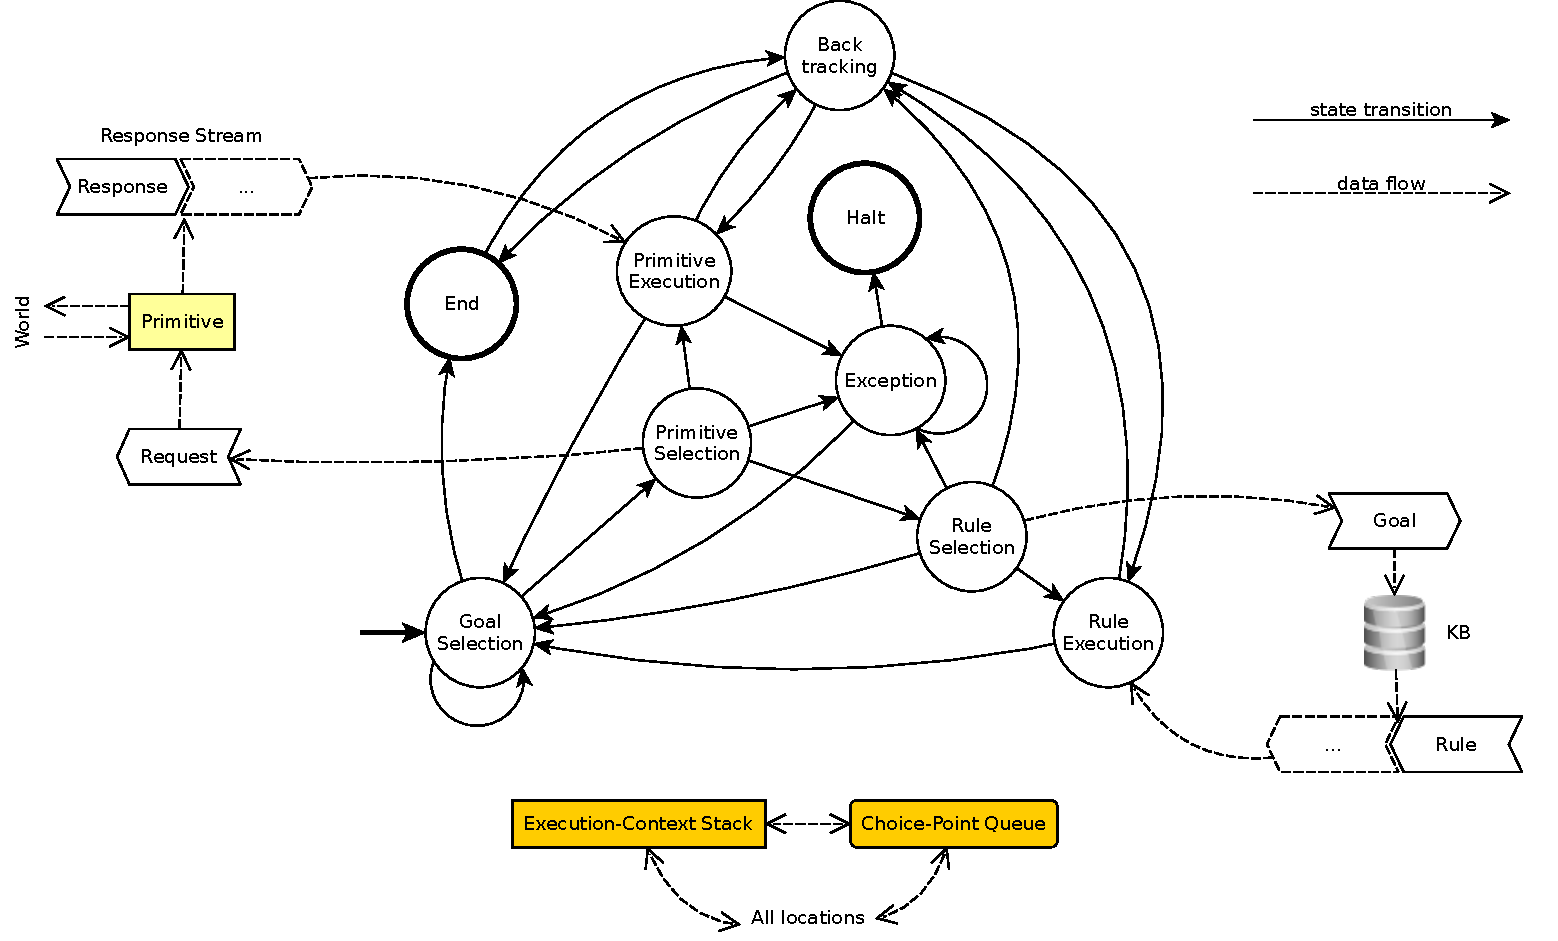
\includegraphics[width=\linewidth]{img/classic-sm.pdf}
    \caption{Overview of our Prolog state machine}
    \label{fig:prolog-fsa}
\end{figure}

The semantics of our Prolog state machine can be described in terms of \emph{states} and \emph{transitions} between them.
%
In this regard, a \emph{state} is a tuple of the form $\langle L, \vect{E}, \vect{C} \rangle$ where
%
\begin{itemize}
    \item $L \in \notableset{L}$ is a location,
    \item $\vect{E} \in \notableset{E}^*$ is an execution-context stack,
    \item $\vect{C} \in \notableset{C}^*$ is a choice-point queue.
\end{itemize}

Accordingly, the state machine semantics is defined as a \emph{labelled transition system} $\langle \notableset{S}, \Lambda, s_0, \longrightarrow \rangle$ where:
%
\begin{itemize}
    \item $\notableset{S}$ is the set of all possible states,
    \item $\Lambda = \{ \tau \} \cup \notableset{X} \cup \Theta $ is a set of labels,
    \item $s_0 \in \notableset{S}$ is the initial state,
    \item $\longrightarrow \subseteq \notableset{S} \times \Lambda \times \notableset{S}$ is a transition relation dictating how state may evolve in time.
\end{itemize}
%
There, transition labels in $\Lambda$ denote relevant observable events, while the anonymous label $\tau$ denotes internal events.
%
Observable events of interest can be, for instance, the production of either a positive or negative solution -- denoted by the corresponding substitution in $\Theta$ -- or the production of an exceptional solution---denoted by the corresponding exception in $\notableset{X}$.
%
In the following, for the sake of notation simplicity, we write $s \transition{\lambda} s'$ instead of $(s, \lambda, s')$ to refer to transitions in $\longrightarrow$.

Assuming that a KB $K$ and a primitive store $I$ are provided, and that the initial state $s_0 \in \notableset{K}$ is always a tuple of the form:
%
\[ \langle \state{Goal Selection},\   [( \varnothing, [g_0], [], [] )],\  [] \rangle \]
%
for some initial goal $g_0$ -- meaning that
%
\begin{inlinelist}
    \item the initial location is always \state{Goal Selection},
    \item the current context initally only contains the empty unifier $\varnothing$ and $g_0$, and
    \item the choice-point queue is initially empty
\end{inlinelist}
%
-- we can \emph{intensionally} define the admissible transitions in $\longrightarrow$ via the following transition rules---each one corresponding to an arrow in \cref{fig:prolog-fsa}.

\subsubsection{Goal Selection}

The purpose of the \state{Goal Selection} location is to decide what to do next depending on which and how many (sub-)goals are in the current execution context.
%
There are three relevant situations handled in this location, by as many transition rules.
%
More precisely, if the current execution context does not contain any goals, this implies either that a new solution should be yielded, or the top execution context should be popped from the stack.
%
Conversely, if the current execution context does hold at least one goal, the automaton commits to that goal---meaning that it tries to prove its truth via subsequent transitions.

Accordingly, the following transition rule handles the case where there is only one last execution context on the stack with no more goals---thus, implying the automaton should move into the \state{End} location and a new solution should be yielded:
%
%More formally:
\[
    \frac{
        E = (\theta, [], [], [])
    }{
        \langle \state{Goal Selection}, [E], \vect{C} \rangle
        \transition{\theta}
        \langle \state{End}, [E], \vect{C} \rangle
    }
\]
The positive or negative solution depends on the $\theta$ substitution of the last execution context $E$, which can be either a unifier or the failed substitution $\bot$. 
In the former case, $\theta$ synthesises all the variable assignments computed so far by the automaton.

Conversely, the following transition rule handles the case where the current execution context has no more goals, but the stack contains
more execution contexts.
%
When this is the case, the automaton simply pops the current execution context from the stack and holds the \state{Goal Selection} location:
\[
    \frac{
        E_0 = (\theta_0, [], [], [])
        \qquad
        E_1 = (\theta_0, \stream{g}, [], [])
        \qquad
        E'_1 = (\theta_1, \stream{g}, [], [])
    }{
        \langle \state{Goal Selection}, [E_0, E_1 \mid \vect{E}], \vect{C} \rangle
        \transition{\tau}
        \langle \state{Goal Selection}, [E'_1 \mid \vect{E}], \vect{C} \rangle
    }
\]
%
Before popping the current execution context $E_0$, the automaton sprads its $\theta_0$ substitution to the parent execution context $E_1$---as $\theta_0$ can contain more assignments than $\theta_1$.

Finally, the following transition rule handles the case in which the current execution context contains a non-empty stream of goals $\stream{g}$.
%
When this is the case the automaton applies the most recent substitution $\theta$ to all the goals in $\stream{g}$ before moving into \state{Primitive Selection} location and tries then to prove the truth of the first sub-goal in $\stream{g}$:
%
\[
    \frac{
        E = (\theta, \stream{g}, [], [])
        \qquad
        E' = (\theta, \stream{g}', [], [])
        \qquad
        \stream{g}' = \apply{\stream{g}}{\theta}
    }{
        \langle \state{Goal Selection}, [E \mid \vect{E}], \vect{C} \rangle
        \transition{\tau}
        \langle \state{Primitive Selection}, [E' \mid \vect{E}], \vect{C} \rangle
    }
\]
%
where by $\apply{\stream{g}}{\theta}$ we mean the application of substitution $\theta$ to all goals in $\stream{g}$.


\subsubsection{Primitive Selection}

The purpose of the \state{Primitive Selection} location is to select a primitive in the primitive store $I$ in order to prove a (sub-)goal---provided a primitive matching the goal's signature exists in $I$.
%
If this is the case, the primitive is triggered and the \emph{first} primitive response is handled.
%
Thus, there are three relevant situations handled in this location, by as many transition rules.
%
A pivotal role in discriminating among situations is played by the first goal $g$ of the current execution context.
%   
If primitive $p$ is indexed in $I$ via signature of $g$, then $p$ is triggered and a response stream is generated in return.
%
Only the first item in the stream, $r$, is consumed.
%
This can be either an exception or a substitution. Each case is handled by a different transition rule.
%
Otherwise, if the signature of $g$ matches no primitive in $I$, no primitive is selected and, via subsequent transitions, a rule for the same goal is searched.

In particular, the following transition rule handles the case where a primitive $p$ is found in $I$ and the first response $r$ is a substitution.
%
When this is the case, a new execution context is pushed on the stack -- for handling the first response --, and a new choice point is appended to queue---for handling any further response.
%
After that, the automaton moves to the \state{Primitive Execution} location.
%
\[
    \frac{
        \begin{array}{c}
            E_0 = (\theta, \stream{g}, [], [])
            \quad
            \stream{g} = [g \mid \stream{g}']
            \quad
            (f, n) = \fx{signature}{g}
            \quad
            (f, n, p) \in I
            \quad
            [r \mid \stream{r}] = p(K, g)
            \\
            r \in \Theta
            \quad
            E_1 = (\theta, \stream{g}, [], [r \mid \stream{r}'])
            \quad
            E_2 = (\theta, \stream{g}, [], \stream{r}')
            \quad
            \vect{C}' = \fx{append}{\vect{C}, [E_2, E_0 \mid \vect{E}]}
        \end{array}
    }{
        \langle \state{Primitive Selection}, [E_0 \mid \vect{E}], \vect{C} \rangle
        \transition{\tau}
        \langle \state{Primitive Execution}, [E_1, E_0 \mid \vect{E}], \vect{C}' \rangle
    }
\]
%
% This implies that there could be other responses in the response stream.
%
% For this reason, a novel choice point is appended to the choice-point queue.
%
% After that, the automaton moves to the \state{Primitive Execution} location.%

Conversely, the following transition rule handles the case in which the first primitive response $r$ is an exception.
%
This implies that there could \emph{not} be any further response in the response stream and the exception needs to be handled.
%
For this reason, the automaton moves into the \state{Exception} location leaving the choice-point queue unaffected:
%
\[
    \frac{
        \begin{array}{c}
            E_0 = (\theta, [g \mid \stream{g}'], [], [])
            \quad
            (f, n) = \fx{signature}{g}
            \quad
            (f, n, p) \in I
            \\
            \left[x \mid \stream{r}\right] = p(K, g)
            \quad
            x \in \notableset{X}
            \quad
            E_1 = (\theta, [g \mid \stream{g}'], [], [x \mid \stream{r}])
        \end{array}
    }{
        \langle \state{Primitive Selection}, [E_0 \mid \vect{E}], \vect{C} \rangle
        \transition{\tau}
        \langle \state{Exception}, [E_1, E_0 \mid \vect{E}], \vect{C} \rangle
    }
\]
%
In this case as well a new execution context is pushed on the stack -- in order to make the exception visible in \state{Exception} --, whereas no new choice point is created.

Finally, the following transition rules handle the case in which a primitive is available in $I$ for the goal $g$.
%
When this is the case, the automaton simply moves into the \state{Exception} location:
%
\[
    \frac{
        E = (\theta, [g \mid \stream{g}'], [], [])
        \qquad
        (f, n) = \fx{signature}{g}
        \qquad
        (f, n, p) \not\in I
    }{
        \langle \state{Primitive Selection}, [E \mid \vect{E}], \vect{C} \rangle
        \transition{\tau}
        \langle \state{Rule Selection}, [E \mid \vect{E}], \vect{C} \rangle
    }
\]

\subsubsection{Primitive Execution}

The purpose of the \state{Primitive Execution} location is to \emph{lazily} handle the response streams produced by primitives.
%
To this regard, there are three relevant situations, handled by as many transition rules.
%
In fact, while consuming a stream of solution responses, the automaton may either encounter an empty stream, or a stream whose first element is either an exception, or a substitution.
%
The latter case is the most interesting one, as the substitution must be kept into account in the next computational steps.
%
Conversely, in the other cases, the response stream is interrupted, even if with different outcomes: while the lack of responses simply provokes backtracking, exceptions need to be handled accordingly.

In particular, the following transition rule handles the case where the first response in the stream is a unifier $\theta'$.
%
When this is the case, $\theta'$ is merged with the current execution context substitution $\theta$ and execution proceeds in the \state{Goal Selection} location.
%
\[
    \frac{
        E = (\theta, [g \mid \stream{g}], [], [\theta', \ldots])
        \qquad
        \theta' \in \Theta - \{ \bot \}
        \qquad
        E' = (\theta \cup \theta', \stream{g}, [], [])
    }{
        \langle \state{Primitive Execution}, [E \mid \vect{E}], \vect{C} \rangle
        \transition{\tau}
        \langle \state{Goal Selection}, [E' \mid \vect{E}], \vect{C} \rangle
    }
\]
%
It is worth to highlight how this transition rule simply consumes a \emph{single} response in the stream.
%
Subsequent responses may be consumed after backtracking.
%
Thus, this is where the lazy semantics of primitives is realised. 

Conversely, the following transition rule handles both the case where the first response in the stream is a failure (i.e. $\bot$), and the case of any empty response stream.
%
In all such cases, the automaton simply moves into the \state{Backtracking} location.
\[
    \frac{
        E = (\theta, \stream{g}, [], \stream{r})
        \qquad
        \stream{r} = [\bot, \ldots] \lor \stream{r} = []
        \qquad
        E' = (\theta, \stream{g}, [], [])
    }{
        \langle \state{Primitive Execution}, [E \mid \vect{E}], \vect{C} \rangle
        \transition{\tau}
        \langle \state{Backtracking}, [E' \mid \vect{E}], \vect{C} \rangle
    }
\]

Finally, the following transition rule handles the case where the first response in the stream is an exception.
%
When this is the case, the automaton simply moves into the \state{Exception} location.
\[
    \frac{
        E = (\theta, \stream{g}, [], [x, \ldots])
        \qquad
        x \in \notableset{X}
        \qquad
        E' = (\theta, \stream{g}, [], [x])
    }{
        \langle \state{Primitive Execution}, [E \mid \vect{E}], \vect{C} \rangle
        \transition{\tau}
        \langle \state{Exception}, [E' \mid \vect{E}], \vect{C} \rangle
    }
\]

\subsubsection{Rule Selection}

The \state{Rule Selection} location is for clauses what the \state{Primitive Selection} location is for primitives.
%
It aims at querying the KB and selecting the rules to be executed to prove a particular (sub-)goal true, provided that no primitive has been selected to the purpose.
%
Accordingly, three transition rules are defined, each one handling a particular situation.
%
The most common situation here is that a number of rules $\stream{r}$ are selected from $K$ in order to solve some goal $g$.
%
However, there is a small set of goals for which a particular treatment is reserved.
%
These are: \texttt{!} (the ``cut''), \texttt{true}, \texttt{fail}, and \texttt{false}.
%
The first two are always considered successful, while the others are always considered failed.

More precisely, the following transition rule takes care of goals such as \texttt{!} and \texttt{true}.
%
As they must always be evaluated successfully, this transition simply makes the automaton move into the \state{Goal Selection} location, after consuming the current goal $g_0$.
%
However, in the particular case of $g_0 \equiv \mathtt{!}$, the transition rule also provokes the \emph{cut} of all choice points, up to the one relative to goal $g_1$ (included):
%
%More formally:
%
\[
    \frac{
        \begin{array}{c}
            E_0 = (\theta_0, [g_0 \mid \stream{g}_0], [], [])
            \qquad
            g_0 \in \{ \mathtt{true}, \mathtt{!} \}
            \qquad
            E_1 = (\theta_1, [g_1, \ldots], \ldots)
            \\
            E'_0 = (\theta_0, \stream{g}_0, [], [])
            \qquad
            \vect{C}' = \fx{cut}{C, g_1}
        \end{array}
    }{
        \langle \state{Rule Selection}, [E_0, E_1 \mid \vect{E}], \vect{C} \rangle
        \transition{\tau}
        \langle \state{Goal Selection}, [E'_0, E_1 \mid \vect{E}], \vect{C}' \rangle
    }
\]
%
where $\f{cut} : \notableset{C^*} \times \notableset{A} \rightarrow \notableset{C^*}$ is the function cutting off choice points, up to a given goal.

Conversely, the following transition rule takes care of goals such as \texttt{fail} and \texttt{false}.
%
As they must always be evaluated successfully, this transition simply makes the automaton move into the \state{Backtracking} location, after consuming the current goal $g$.
%
This transition rule also handles the case where $K$ is queried for all rules whose head unifies with the current goal $g$, but no one is found.
%
\[
    \frac{
        E = (\theta, [g, \ldots], [], [])
        \qquad
        g \in \{ \mathtt{false}, \mathtt{fail} \} \lor \fx{get}{K, g} = []
    }{
        \langle \state{Rule Selection}, [E \mid \vect{E}], \vect{C} \rangle
        \transition{\tau}
        \langle \state{Backtracking}, [E \mid \vect{E}], \vect{C} \rangle
    }
\]

Finally, the following transition rule handles the general case where $K$ is queried for all rules $\stream{h}$ whose head unifies with the current goal $g$.
%
Assuming that $\stream{h}$ contains at least one rule $h$, the automaton must then move to location \state{Rule Execution}, after pushing a new execution context on the stack -- aimed at handling $h$ --, and adding a new choice point to the queue---aimed at handling any further rule in $\stream{h}$:
%
%More formally:
%
\[
    \frac{
        \begin{array}{c}
            E_0 = (\theta, \stream{g}, [], [])
            \quad
            \stream{g} = [g \mid \stream{g}']
            \quad
            g \in \notableset{A} - \{ \mathtt{true}, \mathtt{false}, \mathtt{fail}, \mathtt{!} \}
            \\
            \fx{get}{K, g} = \stream{h}
            \quad
            \fx{refresh}{\stream{h}} = [h \mid \stream{h}']
            \\
            E_1 = (\theta, \stream{g}, [h \mid \stream{h}'], [])
            \quad
            E_2 = (\theta, \stream{g}, \stream{h}', [])
            \quad
            \vect{C}' = \fx{append}{\vect{C}, [E_2, E_0 \mid \vect{E}]}
        \end{array}
    }{
        \langle \state{Rule Selection}, [E_0 \mid \vect{E}], \vect{C} \rangle
        \transition{\tau}
        \langle \state{Rule Execution}, [E_1, E_0 \mid \vect{E}], \vect{C}' \rangle
    }
\]
%
where $\f{refresh} : \notableset{H}^* \rightarrow \notableset{H}^*$ is a function refreshing all variables of all clauses in a clause stream/list.

\subsubsection{Rule Execution}

The \state{Rule Execution} location is for clauses what the \state{Primitive Execution} location is for primitives.
%
Thus, the purpose of this location is to \emph{lazily} handle the rule streams produced by KB.
%
Accordingly, two transition rules are defined, each one handling a particular situation.
%
In both situations, the current execution context is assumed to carry a non-empty rule stream to be handled.
%
One situation concerns the case where the first rule in the stream has a head matching the current context goal.
%
In this case, the execution can go on and focus on the body of that rule.
%
The other situation concerns the opposite case, where execution must proceed with backtracking.
%
% In any case, the automaton cannot be in location \state{Rule Execution} while the rule stream of the execution context is empty.

Accordingly, the following transition rule handles the first situation.
%
The current execution context's first goal is $g$ and the first rule is $h$. 
%
Provided that the head of $h$ unifies with $g$, and letting $\theta'$ be their unifier, the current execution context is updated in such a way that the new substitution is $\theta \cup \theta'$ and the new goal stream contains all the atoms from the body of $h$, subject to the substitution $\theta'$.
%
After that, the automaton moves to the \state{Goal Selection} location.
\[
    \frac{
        \begin{array}{c}
            E = (\theta, [g \mid \stream{g}], [h, \ldots], [])
            \quad
            h = (a \leftarrow a_1, \ldots, a_n)
            \quad
            \theta' = \fx{mgu}{g, a} \neq \bot
            \\
            E' = (\theta \cup \theta', [\apply{g_1}{\theta'}, \ldots, \apply{g_n}{\theta'}], [], [])
        \end{array}
    }{
        \langle \state{Rule Execution}, [E \mid \vect{E}], \vect{C} \rangle
        \transition{\tau}
        \langle \state{Goal Selection}, [E' \mid \vect{E}], \vect{C} \rangle
    }
\]

Conversely, the following transition rule handles the case where the head of $h$ does not unify with $g$.
%
In this case, the automaton simply moves into the \state{Backtracking} location.
%
\[
    \frac{
        E = (\theta, [g \mid \stream{g}], [h, \ldots], [])
        \quad
        h = (a \leftarrow \ldots)
        \quad
        \fx{mgu}{g, a} = \bot
        \quad
        E' = (\theta, [g \mid \stream{g}], [], [])
    }{
        \langle \state{Rule Execution}, [E \mid \vect{E}], \vect{C} \rangle
        \transition{\tau}
        \langle \state{Backtracking}, [E' \mid \vect{E}], \vect{C} \rangle
    }
\]

\subsubsection{Backtracking}

The \state{Backtracking} location is the key point where the lazy consumption of rules and responses streams is performed by Prolog solvers.
%
More precisely, this is where the choice points previously accumulated by the automaton in the choice-points queue are handled.
%
Following this purpose, the \state{Backtracking} location may encounter three relevant situations, all depending on the content of the queue.
%
The first situation concerns the case of the queue is empty, meaning that a new negative solution should be produced by the solver.
%
The other situations concern the cases where the next choice point is carrying a non-empty rule or primitive response stream, respectively.
%
In these cases, the automaton should move into either the \state{Rule} or \state{Primitive Execution} locations, in order to go on with resolution and consume the next rule or response.

Accordingly, the following rule handles the case where the choice-point queue is empty and the and the automaton should just move into the \state{End} final location, yield a new negative solution $\bot$.
%
\[
    \frac{
        %
    }{
        \langle \state{Backtracking}, \vect{E}, [] \rangle
        \transition{\bot}
        \langle \state{End}, \vect{E}, [] \rangle
    }
\]

Conversely, the following rule handles the case where the next choice point $C$ in the queue is an execution context carrying a non-empty primitive response stream $\stream{r}$.
%
When this is the case, the automaton simply adopts $C$ as the next execution context, popping it from the choice-point queue and moving into the \state{Primitive Execution} location.
%
\[
    \frac{
        C = [(\theta, \stream{g}, [], \stream{r}), \ldots]
        \qquad
        \stream{r} \neq []
    }{
        \langle \state{Backtracking}, \vect{E}, [C \mid \vect{C}] \rangle
        \transition{\tau}
        \langle \state{Primitve Execution}, C, \vect{C} \rangle
    }
\]

Finally, the following rule handles the case where the next choice point $C$ in the queue is an execution context carrying a non-empty rule stream $\stream{h}$.
%
When this is the case, the automaton simply adopts $C$ as the next execution context, popping it from the choice-point queue and moving into the \state{Rule Execution} location.
%
\[
    \frac{
        C = [(\theta, \stream{g}, \stream{h}, []), \ldots]
        \qquad
        \stream{h} \neq []
    }{
        \langle \state{Backtracking}, \vect{E}, [C \mid \vect{C}] \rangle
        \transition{\tau}
        \langle \state{Rule Execution}, C, \vect{C} \rangle
    }
\]

\subsubsection{Exception Handling}

The \state{Exception} location has the purpose of managing exceptions possibly raised by primitive responses in the Standard Prolog way---i.e. by climbing the proof tree towards the root, looking for a \pl{catch/3} (sub-)goal whose second argument unifies with the raised exception and setting its third argument as the next sub-goal to be proved.

Following this purpose, the \state{Exception} location may encounter two notable situations.
%
In both ones, the current execution is assumed to be carrying an exception $x \in \notableset{X}$.
%
The first situation concerns the case where the exception can be \emph{caught} since there exists on the stack an execution context of the form \pl{catch/3} which may intercept the exception and let resolution continue.
%
The second situation concerns the opposite case where the exception \emph{cannot} be caught -- since no such an execution context is contained into the stack -- and resolution must be therefore interrupted.

In particular, the following transition rule handles the first situation where an execution context $E'$ exists on the stack whose first goal is $\mathtt{catch}(g_1, g_2, g_3)$.
%
When this is the case, we denote by $\theta'$ the MGU among $x$ and $g_2$.
%
Then, the automaton pops from the stack all execution contexts up to $E'$ (included), pushes a new execution context carrying $g_3$ as the first goal, and moves into the \state{Goal Selection} location.
%
\[
    \frac{
        \begin{array}{c}
            E = (\theta, [g \mid \stream{g}], [], [x, \ldots])
            \quad
            x \in \notableset{X}
            \quad
            E' = (\vartheta, [\mathtt{catch}(g_1, g_2, g_3), \ldots], \stream{h}, \stream{r})
            \\
            \theta' = \fx{mgu}{x, g_2} \neq \bot
            \quad
            \theta'' = \vartheta \cup \theta'
            \quad
            E'' = (\theta'', [g_3 / \theta''], [], [])
        \end{array}
    }{
        \langle \state{Exception}, [E, \ldots, E' \mid \vect{E}], \vect{C} \rangle
        \transition{\tau}
        \langle \state{Goal Selection}, [E'' \mid \vect{E}], \vect{C} \rangle
    }
\]

Conversely, the following transitions rule handles the opposite situation where no execution context on the stack carries $\mathtt{catch}(g_1, g_2, g_3)$ as the first goal---or, if it does, $g_2$ does not unify with $x$.
%
When this is the case, the automaton simply moves into the \state{Halt} location, yielding an exceptional solution to the users.
%
\[
    \frac{
        \begin{array}{c}
            E = (\theta, [g \mid \stream{g}], [], [x, \ldots])
            \qquad
            x \in \notableset{X}
            \\
            \vect{E} \neq [E, \ldots, (\vartheta, [\mathtt{catch}(g_1, g_2, g_3), \ldots], \stream{h}, \stream{r}), \ldots]
        \end{array}
    }{
        \langle \state{Exception}, [E \mid \vect{E}], \vect{C} \rangle
        \transition{x}
        \langle \state{Halt}, [E \mid \vect{E}], \vect{C} \rangle
    }
\]

\subsubsection{Next Solutions}

Both the \state{End} and \state{Halt} locations are final, meaning that the automaton reaches them immediately after the production on a novel solution---be it positive, negative, or exceptional.
%
However, while the \state{Halt} location is a sink certainly provoking the automaton termination, the \state{End} state may allow the execution to be resumed.
%
In particular, when the automaton is in location \state{End}, the users may trigger the automaton again looking for further solutions---which \emph{may} be available if the choice-point queue is not empty.

Accordingly, the following transition rule handles the case where the automaton execution is resumed: once in location \state{End} the automaton may move back into location \state{Backtracking}, provided that the current choice-point queue $\vect{C}$ is non-empty.
%
\[
    \frac{
        \vect{C} \neq []
    }{
        \langle \state{End}, \vect{E}, \vect{C} \rangle
        \transition{\tau}
        \langle \state{Backtracking}, \vect{E}, \vect{C} \rangle
    }
\]
%
Thus, the automaton actually terminates in location \state{End} only when the choice-point queue is empty.


\end{document}
